В ходе измерений были получены данные \ref{fig:expD12}. Красной кривой отмечен спектр при наличии насыщающего пучка, черной кривой соответствует спектр в отсутствии насыщающего пучка. 

Более подробная картинка вблизи резонанса D${}_1$ и D${}_2$ разницы двух кривых приведена в дополнение, параметры оценены из аппроксимации суммой лоренцовых контуров. 


\begin{figure}[h]
    \centering
    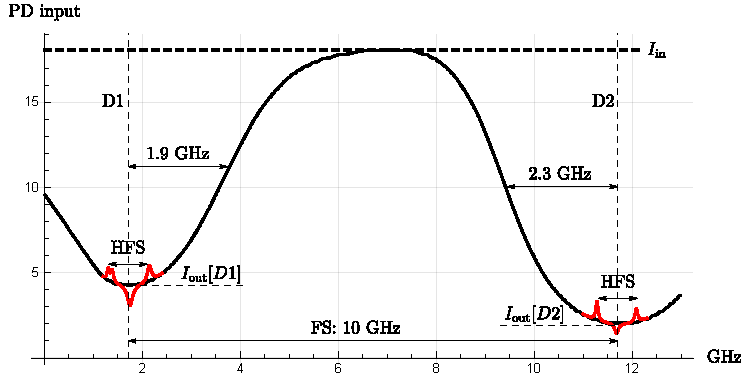
\includegraphics[width=0.7\textwidth]{D:\\Kami\\git_folder\\notes_5sem\\rqc\\data_processing_1\\exp_D12_v2.pdf}
    \caption{Полученный спектр для D1 и D2}
    \label{fig:expD12}
\end{figure}


Параметры наблюдаемого спектра приведены в таблице \ref{tab:params1}.
Расстояние между линиями D$_1$ и D$_2$ было взято за эталон частоты.

\begin{table}[h]
    \centering
    \caption{Параметры полученного спектра}
    \begin{tabular}{c|cc}
    \toprule
       & $\beta_0$ & $K$  \\
   \midrule
    D$_1$ & 0.24 & 7.3 \% \\
    D$_2$ & 0.11 & 6.2 \% \\
    \bottomrule
    \end{tabular}
    \label{tab:params1}
\end{table}



